\chapter{Review of Related Literature}
\label{chap:literature_review}

This chapter discusses the foundational theories, real-world applications, and methodological frameworks that are related to traffic network paradoxes. Reviews the core concepts of the Braess Paradox while situating these concepts within the local context of the Iloilo City Transportation System

% \include{chapter_II/rrl_subsections/2.1}
% \include{chapter_II/rrl_subsections/2.1.1}

\section{Graph Theory}
\label{chap:graph_theory}

Networks made up of nodes and connections are found in a wide range of applications. They can model physical and conceptual systems. They can also represent more abstract relationships, such as interactions within ecosystems, database structures, and even program logics \parencite{gross2018graph}. To formally study and analyze these types of relationships, the concept graph theory is utilized.
In the fields of mathematics and computer science, graph theory refers to the framework for modeling relationships between pairs of objects. A graph consists of two sets called vertices or nodes and edges which connect them \parencite{prath}(Prathik et al., 2016). Formally, a graph G = (V,E) is defined as an ordered pair, namely V and E. The elements of V are referred to as vertices, while the elements of E are called edges. Each edge is associated with one or two vertices, referred to as its endpoints \parencite{chang2002introduction}. 

Graphs serve as foundational tools for mapping complex networks, like data organization and communication pathways (Prathik et al., 2016). For example, in transportation networks, traffic systems can be effectively modeled as graphs in which the physical intersections act as nodes and the connecting roads serve as edges. In public transportation systems, stations and stops can be referred to as nodes whereas the travel routes that connect them are referred to as edges. By applying the graph theory to these networks, transportation planners can optimize bus or railroad to accommodate passenger timetable and demand, keeping public transportation a viable and effective option for commuters \parencite[]{} (Reddy et al., 2024). 



\section{Traffic Congestion in Urbanized Cities}
\label{chap:traffic_congestion}

Traffic congestion does not have a single definition. \textcite{aftabuzzaman2007measign} categorized the definitions into three groups: demand capacity, delay-travel time, and cost. This study notes the definition of congestion by Akthar \& Modipour (2021) as the imbalance between increased traffic flow and limited road capacity, with greater emphasis on demand capacity-related considerations.
Traffic congestion can be triggered by various factors, including traffic incidents, road works, weather conditions, and special events. These causes are classified into recurring and nonrecurring congestions as shown in Figure 1 \parencite{jilani2023systematic}.

\begin{figure}[ht]
    \centering
    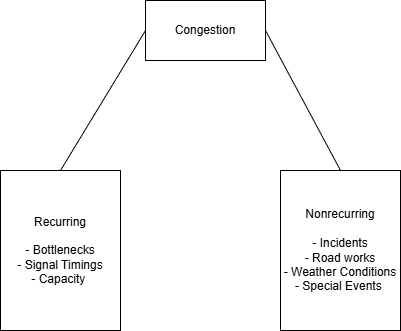
\includegraphics[scale=0.6]{figures/figure-1.png}
    \caption{Classification of Congestion. Adapted from Jilani et al. (2023)} 
    \label{fig:congestion_classification}
\end{figure}

In the Philippines, specifically in Metro Manila, the rising vehicle sales are cited as one of the factors in the increased road traffic, mainly due to inefficient public transportation systems in the metro \parencite{jica2025jica}. As a result, traffic congestion affects components in the daily transport system. In the study of \parencite{gonzalez2021understanding}, the results show that congestion is highly correlated with accidentality, with congestion having a significant effect on accidentality rates.

Additionally, \parencite{onyeneke2018modeling} added that there is a strong positive correlation in the number of accidents to the number of registered vehicles, such as the observation that the increase of registered vehicles leads to an increase in congestion, increasing injuries and fatalities. Another effect that traffic congestion brings forth is the distribution of pollution. As stated in a literature survey from \textcite{marve2016survey}, cars in traffic produce large quantities of carbon emissions that can cause localized problems such as deficient air quality within a community. Vehicle emissions are dependent on the vehicles motion; thus, the erratic motion of cars results in a higher rate of fuel burning compared to smooth travel. Also, high fuel consumption links in a higher cost to the commuter’s money to purchase more fuel.

Urbanized cities in the Philippines, such as Metro Manila, Cebu City, and Davao City, have an ongoing struggle with congestion due to their rapid urbanization, increased vehicle registration, and limited enforcement capabilities \parencite{tuco2025traffic}. As recognized by the Bureau of Local Government Finance (2025), Iloilo City ranks second among the highly urbanized cities in the Philippines. This continuous rise in urbanization demonstrates the symbiotic relationship between transportation and urbanization, as described by \parencite{rodrigue2024transportation}, where urban mobility and transportation systems shape the growth and structure of cities.

On a local scale, Landoy et al. (2012, as cited in Sosuan \& Fillone, 2014), the vehicular speed-density-flow relationships of primary roads in Iloilo City are the National Highway and Lopez Jaena St., Diversion Road, General Luna St., and J.M. Basa St., respectively. By using the Greenshield model and the Greenberg model, the result indicates that it shows an approach to congestion of roads by the Highway Capacity Manual.

\subsection{Traffic Management Systems}
\label{chap:traffic_management_systems}

In recent developments, traffic management systems have centered around the modern technology of the Intelligent Transport Management System. As defined by \textcite{chowdhuryits}, Intelligent Transport Systems or ITS is the use of information and communication technologies, such as control and information systems, to integrate communications and data processing technologies in traffic. Additionally, the integration of systems addresses improving the mobility of people, managing traffic congestion, and aligning with transport policy goals and objectives.

Specific to the Philippines, the Metropolitan Manila Development Authority inaugurated an urban traffic management system from INDRA in 2014 \parencite{indra2014urban}. INDRA incorporated a system core in INDRA’s 997 Hermes smart traffic management system. The intelligent transport system comprises a centralized stoplight system with 90 stoplight intersections having over 600 detectors at each intersection, and a CCTV system. These systems are then managed by a software based on an algorithm that uses real-time data to optimize a traffic plan. The CCTV system is then used to project in the control center of 35- 50-inch monitors. According to the MMDA, the intelligent traffic system by INDRA has observed cost savings, reduced polluting elements, improved road safety, and decreased hold-up times within Metro Manila \parencite{indra2014urban}.

A study by \textcite{cueto2024intelligent} incorporated prediction and simulation through predicting the traffic volume by 10 years to which is used in a simulation model through SUMO. By predicting the traffic congestion in the future, the study can be used to manage future traffic demands. As noted by the result of the study, even if the current ITS in Metro Manila uses ITS applications such as CCTVs, monitor control, and traffic management tools, yet “to explore the use of traffic simulation softwares as a means to improve and study the current traffic situation in their city.”

So far, the application of the Braess Paradox in the traffic management system is an area that needs exploration and improvement. A relevant study conducted by \textcite{joseph2022applications} has implemented Braess’ paradox in a traffic management software that provides the driver with the most efficient route to decrease traffic and minimize commute time, as opposed to giving the same detour route if traffic congestion exists. The study showed that by using the Franke Wolfe algorithm to train its Neural Network, the software identified new routes according to the Braess paradox, which then maximizes efficiency and decreases travel time for the driver. While the study shows the efficiency in the application of the Braess’ Paradox to finding an optimal route, its application is limited in treating the road network as a fixed entity. Thus, it does not observe the principle of the paradox in which structural modification, such as a permanent removal of a road, improves the flow of traffic.

\section{Transportation Network Equilibrium Models}
\label{chap:equilibrium_models}

Transportation Network Models (TNM) is the classical approach for traffic flow analysis, which is rooted in optimization, and treats traffic as a divisible, static flow moving through a system seeking a stable state. The primary goal is to mathematically calculate the User Equilibrium (UE), a state where no driver can unilaterally find a faster travel time by changing routes. This was established by the foundational work of Braess (1968, as translated by Braess et al., 2005).

Following the graph-theoric framework established in Section 2.1, transportation networks are modeled as direct graphs where physical intersections are represented as vertices and road segments as edges. In the Philippine context, this graph-theoric approach has been utilized to model traffic congestions at major urban junctions, such as those along Taft Avenue in Manila, where edges are assigned weights corresponding to travel distance or traffic volume \parencite{abanes2017traffic}. Using the graph-theoric framework, Braess (1968, as translated by Braess et al., 2005), in his seminal work, not only introduced the paradox but also provided the mathematical method for finding the “critical flow” by solving a convex optimization problem.

However, while mathematically robust, this model suffers a “fidelity gap” as its simple functions fail to account for the severe, non-linear impact of real-world intersection queuing. Modern research refines this approach as seen in the work of \textcite{burov2021detecting}, where they directly address this gap by proposing an “extended graph representation”, which introduces “phantom links”, which are virtual segments that represent queuing into the optimization model. This allows for a classical convex optimization model to account for the queuing delays, making it more accurate for detecting Braess routes in real-world networks.

\subsection{User Equilibrium (UE) and System Optimum (SO)}
\label{chap:UE_and_SO}

In transportation modeling, traffic assignment is traditionally cetogirized into two primary frameworks derived from Wardrop's principles, that is, the User Equilibrium and System Optimum \parencite{mora}(Morandi, 2023).

\subsubsection{User Equilibrium (UE)}
\label{chap:UE}

A widely accepted assumption in transportation and telecommunications network studies is that travelers or data packets will always take what seems to the fastest route given current traffic conditions (Correa \& Stier-Moses, 2011). As a result, all utilized routes share the same minimized travel time, whereas unused routes have travel times that are equal to or longer than those routes being used (Chen et al., 2024). Formally conceptualized by Wardrop in 1852, this concept is now known as the Wardrop (or user) equilibrium.

In User Equilibrium (UE), uncoordinated drivers choose routes that minimize their overall travel time. Thus, the term "selfish routing". In this state, users cannot improve their travel times by changing routes, hence a Nash Equilibrium (Youn et al., 2008). Computationally, the algorithm finds the equilibrium flows ($f_{ij}^{NE}$) by minimizing the following function:

\begin{equation}
    \tilde{\mathcal{C}} = \sum_{\text{link}(i,j)} \int_{0}^{f_{ij}} l_{ij}(f') \, df'
    \label{eq:beckmann_objective}
\end{equation}

\subsubsection{System Optimum (SO)}
\label{chap:SO}

Contrary to the User Equilibrium (UE), the System Optimum (SO) represents a state where traffic is directed to minimize the total travel time across the entire network. This approach is characterized by a centralized routing strategy aimed at achieving the most beneficial state for society as a whole (Youn et al., 2008). Mathematically, the socially optimal flows ($f_{ij}^{SO}$) are determined by minimizing the overall cost to society per unit time \textit{C}:

\begin{equation}
    \mathcal{C} = \sum_{\text{link}(i,j)} l_{ij}(f_{ij}) \cdot f_{ij}
    \label{eq:system_optimum}
\end{equation}

However, achieving system optimum often results in travel time disparities among users traveling between the same origin and destination. This happens because the main priority of a System Optimized network is reducing the system's travel time over individual costs. While the System Optimum (SO) represents the most efficient traffic assignment, it is inherently unstable and unfair as users are less likely to comply with routing prescriptions (Klein et al., 2018).

\subsection{The Bureau of Public Roads (BPR) Function}
\label{chap:BPR}

In modeling traffic behavior, transportation networks must take into account how delays depend on the volume of flow on each link. A widely utilized tool for this purpose is the Bureau of Public Roads (BPR) function, which serves as a standard model in civil engineering for calculating travel delays (Youn et al., 2008).

According to Youn et al. (2008), the delay ($l_{ij}$) on a directed link from node $i$ to node $j$ is calculated as follows:

\begin{equation}
    l_{ij} = \frac{d_{ij}}{v_{ij}} \left[ 1 + \alpha \left( \frac{f_{ij}}{p_{ij}} \right)^\beta \right]
    \label{eq:BPR_function}
\end{equation}

where:

\begin{itemize}
    \item $\frac{d_{ij}}{v_{ij}}$ represents the time needed to travel the distance ($d_{ij}$) at the permitted speed limit ($v_{ij}$) on an empty road.
    \item $f_{ij}$ represents the current number of vehicles utilizing the link per unit of time.
    \item $p_{ij}$ represents the maximum traffic volume the road segment can handle.
    \item $\alpha$ and $\beta$ determines the steepness of the delay; as traffic volume ($f_{ij}$) approaches capacity ($p_{ij}$), travel times increase significantly.
\end{itemize}

Under low traffic volumes, the BPR function remains relatively flat. Contrarily, when traffic flow increases and approaches the capacity of the road segment, the travel time begins to rise significantly.  After establishing the relationship between the travel time of a link and traffic flow through the BPR function, iterative procedures are typically adopted to determine the equilibrium traffic distribution. Within this framework, the Frank-Wolfe algorithm and the Methods of Succesive Averages (MSA) are frequently used in calculating these assignments (Sven Maerivoet \& Moor, 2005)


\subsection{Price of Anarchy}
\label{chap:PoA}

    In the context of transportation networks, Youn et al. (2008) introduced the Price of Anarchy (PoA) as the ratio of the total travel cost at the Nash Equilbrium (User Equilibrium) and the total cost at the social optimum. This metric provides an indication of the inefficiency of decentralization.

The PoA is calculated as follows:

\begin{equation}
    PoA = \frac{\sum_{i,j} l_{ij}(f_{ij}^{NE}) \cdot f_{ij}^{NE}}{\sum_{i,j} l_{ij}(f_{ij}^{SO}) \cdot f_{ij}^{SO}}
    \label{eq:poa_calculation}
\end{equation}

where

\begin{itemize}
    \item $l_{ij}(\cdot)$ is the delay function representing the time needed to travel along link $(i, j)$.
    \item $f_{ij}^{NE}$ denotes the traffic flow on link $(i, j)$ at the Nash Equilibrium (User Equilibrium)
    \item $f_{ij}^{SO}$ represents the socially optimal traffic flow on link $(i, j)$.
    \item $\sum l_{ij}(f_{ij}^{NE}) \cdot f_{ij}^{NE}$ represents the total network travel cost in a decentralized state.
    \item $\sum l_{ij}(f_{ij}^{SO}) \cdot f_{ij}^{SO}$ represents the total network travel cost in the most efficient state possible.
\end{itemize}

As demonstrated in the simulations by Youn et al. (2008), a PoA greater than 1 indicates that uncoordinated individuals are wasting a portion of their travel time. In Boston, the PoA reachead approximately 1.30, suggesting that uncoordinated drivers waste 30\% of their potential travel time. 

\section{Theoretical Framework of the Braess Paradox}
\label{chap:theoretical_bp}

Transportation and communication networks serve as primary examples of physical networks. In this framework, nodes represent locations in space, while links represent the pathways between them. These networks provide the foundational infrastructure on which a portion of social and economic activities rely. While it may appear intuitive that expanding the capacity of a traffic or communication network, by introducing new edges or expanding existing ones, would improve efficiency, this assumption does not always hold. In 1968, Braess demonstrated that, paradoxically, the addition of a new link that connects two parallel routes between the same origin and destination can actually increase the overall travel cost experienced by all network users. This counterintuitive result was later identified as the Braess Paradox (Rapoport et al., 2009).  

As explained by Nagurney \& Nagurney (2020), user behavior is typically described in terms of user-optimization or system-optimization, which is based on Wardrop’s (1952) two principles of travel behavior. In a user-optimized network, each user “selfishly” selects the route that would minimize their own travel time. Equilibrium is reached when all used paths between an origin and destination have equal and minimal travel costs, leaving users no incentive to change routes. Conversely, in a system-optimized network, a central controller is responsible for routing traffic so that the network's travel cost is minimized. BP specifically emerges under user-optimizing conditions, where “selfish” choices lead to increased congestion and longer travel times.

Moreover, Nagurney \& Nagurney (2020) describe that the foundational model used by Braess is a simple four-node network, shown in Figure 2, consisting of an origin, a destination and two intermediate nodes. In this model, all users share a single origin/destination (OD) pair, that is, moving from node one (1) to node four (4). Each link represents a segment of the road network whose travel cost depends on congestion, which means that as the number of users increases, so does the travel time on that link. Users can reach the destination through two alternative routes: links \emph{a} to \emph{c} and links \emph{b} to \emph{d}.

In this set-up, users act under user-optimized conditions, distributing themselves between the two available routes until equilibrium is reached, where users can no longer change routes. To demonstrate the paradox, Nagurney \& Nagurney (2020) described a modification of the four-node network in which an additional link \emph{e} was added between two intermediate nodes. While this newly opened path appears to improve traffic flow and reduce travel times, it will ultimately lead to increased travel costs for all users. As users act “selfishly” to minimize their own travel time, the network reaches a new equilibrium in which the total travel cost for everyone increases relative to the original configuration.

\begin{figure}[ht]
    \centering
    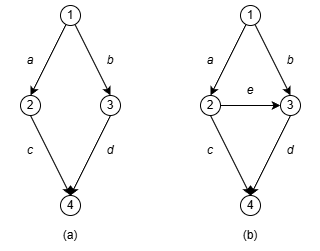
\includegraphics[scale=0.6]{figures/figure-2.png}
    \caption{Four-Node Transportation Network before and after Link Addition. Adapted from Nagurney and Nagurney (2020)} 
    \label{fig:four_node_model}
\end{figure}

Hwand \& Cho (2015) revisited the classical BP and demonstrated that removing a link can enhance overall network performance. In their study, a generalized inverse method was developed to analyze cases that involve non-unique equilibrium path flows,  a condition that is commonly found in real transportation networks. In classical formulations of the BP, the network is typically assumed to have a unique equilibrium, that is, only one possible traffic distribution across routes that satisfies user-equilibrium conditions. To extend this framework, Hwang \& Cho (2015) proposed a testing matrix that determines whether a network will exhibit paradoxical behavior following structural modification, that is, the addition or removal of a link. 

When this matrix is positive semi-definite, at least one OD pair experiences a decrease in total travel cost. Through numerical analysis, the authors demonstrated that the addition of a new link between two nodes increased the total travel cost, while the removal of that same link subsequently reduced it (Hwang \& Cho, 2015). 	

\subsection{Braess Paradox in Traffic Networks}
\label{chap:bp_traffic_networks}

The BP is famously applied to traffic networks, in which it is shown that closing up roads can help in speeding up traffic. The paradox has been observed in complex urban transportation systems from around the world. In Seoul, South Korea, the Cheonggye Expressway was closed due to its restoration project. As a result, the traffic congestion around the city was more efficient, and later the elevated highway was removed to restore the Cheonggyecheon River below it (Easley \& Kleinberg, 2010). This restoration was also the catalyst for eco-friendly urban design, economic development, and preservation of history and the city’s natural environment (Harvard University Graduate School of Design, 2023).

In 2010, New York City Mayor Michael R. Bloomberg initiated an experimental project that involved closing sections of Broadway, particularly in Times Square and Herald Square, to evaluate the effects on traffic and pedestrian movement. While the project fell short of its objective to improve traffic flow, with traffic along Seventh Avenue moving only 4\% faster compared to the expected 17\% improvement, it still led to notable gains in pedestrian safety and foot traffic within the area (Grynbaum, 2010). 

\subsection{Empirical Evidence and Simulation-Based Investigations of the Braess Paradox}
\label{chap:bp_empirical}

While the BP was initially a theoretical framework, numerous studies have since attempted to observe its presence in real-world networks using various simulation tools and varying traffic conditions. Youn et al. (2008), for example, analyzed the principal roads of Boston, New York, and London using data derived from Google Maps to identify principal road segments and intersections. Employing the Bureau of Public Roads (BPR) function, they then compared the traffic patterns produced under a user-optimized system with those generated under a system-optimized configuration. Their findings revealed several locations where closing a road segment reduced total travel time, specifically six in Boston, seven in London, and twelve in New York, offering empirical evidence of the existence of the BP in actual urban networks. 

Rapoport et al. (2009), approached the BP from an experimental perspective, conducting their study in a large computerized laboratory. In their experiment, participants were given the opportunity to select routes in a simplified traffic network that replicated the structure of the classic Braess model. Each participant was compensated according to the travel time associated with the route they selected: the shorter the travel time, the higher the reward. This structure encouraged participants to look for routes that would minimize their individual travel times. When an additional link was introduced, the participants gravitated towards the routes that appeared optimal but collectively resulted in higher travel times, illustrating the BP. Contrarily, removing the additional link decreased overall travel time for the group, showing the BP’s inverse effect. These findings show that selfish route choices can generate congestion counterintuitively even within simplified experimental networks.

Thunig and Nagel (2016) utilized ABM via the MATSim framework to study the BP in dynamic, queuing-based scenarios. Unlike previous studies that treated traffic as a fluid flow, this approach revealed that the paradox only emerges under certain network conditions and disappears under others. In particular, they found that when congestion does not spill back upstream along links, the increase in travel time caused by adding a new link remains limited. However, when spillbacks occur–where queues grow long enough to block intersections and restrict mobility on preceding road segments–the paradox becomes more severe. Their results show that models unable to represent spillback effects tend to underestimate the magnitude of the BP. 

Pas and Principio (1997) explored how economic incentives could alter route choice behaviors to mitigate the effects of the BP. Their research utilized mathematical equilibrium modeling to demonstrate that the negative effects of the BP could be neutralized without physical road closures. Instead, they proposed the application of marginal cost pricing, specifically, by placing a targeted toll on the paradoxical link. This intervention effectively modifies the user’s cost function, disincentivizing the “selfish” route and forcing the network to be system-optimized.

Taken together, these various approaches demonstrate the complex nature of urban traffic congestion. Although the objectives, modeling tools, and operational settings differ across studies, they collectively illustrate how the BP has developed from a theoretical framework into a phenomenon observable in practice.  Table 1 presents a summary of their distinctive findings.

\begin{landscape}

\begin{table}[p]
    \hspace*{2cm}% 
    \begin{minipage}{\dimexpr\linewidth-2cm\relax}
        \caption{Summary of Key Empirical and Simulation Studies on the BP} 
        \vspace{0.25cm}
        \begin{tabularx}{\linewidth}{|p{2.5cm}|X|X|X|X|}
        \hline
        \textbf{Author(s) \& Year} & \textbf{Objectives / Goals} & \textbf{Factors \& Conditions} & \textbf{Simulation Tools / Methodology} & \textbf{Significant Findings} \\
        \hline
        Pas \& Principio (1997) & To explore economic interventions to mitigate BP without physical infrastructure changes. & Factors: Cost Functions, Tolls. \newline \newline Conditions: Economic equilibrium models with variable pricing. & Mathematical Equilibrium Modeling: Cost function manipulation. & The negative effects of BP can be neutralized via marginal cost pricing (targeted tolls) on the paradoxical link, forcing the network toward a system-optimum without requiring physical road closures. \\
        \hline
        Youn, Gastner, \& Jeong (2008) & To identify the presence of the Braess Paradox (BP) in real-world urban road networks. & Factors: Network Topology, Travel Time. \newline \newline Conditions: Real-world principal road networks of Boston, New York, and London. & Topological Analysis: Bureau of Public Roads (BPR) function using data derived from Google Maps. & Provided empirical evidence of BP in actual cities; identified specific road segments (6 in Boston, 7 in London, 12 in NYC) where closure would theoretically reduce total travel time. \\
        \hline
        \end{tabularx}
    \end{minipage}
\end{table}

\begin{table}[p]
    \ContinuedFloat
    \hspace*{2cm}% 
    \begin{minipage}{\dimexpr\linewidth-2cm\relax}
        \caption[]{Summary of Key Empirical and Simulation Studies on the BP (Continued)}
        \vspace{0.25cm}
        \begin{tabularx}{\linewidth}{|p{2.5cm}|X|X|X|X|}
        \hline
        \textbf{Author(s) \& Year} & \textbf{Objectives / Goals} & \textbf{Factors \& Conditions} & \textbf{Simulation Tools / Methodology} & \textbf{Significant Findings} \\
        \hline
        Rapoport et al. (2009) & To validate the behavioral assumptions of BP (selfish routing) in a controlled setting. & Factors: Human Route Choice, Financial Incentives. \newline \newline Conditions: Controlled laboratory environment with "selfish" payout structures. & Experimental Game: Computerized route-selection simulation with human participants. & Confirmed that "selfish" human behavior triggers the paradox; adding a link increased collective travel time, while removing it decreased travel time, validating the inverse effect of BP. \\
        \hline
        Thunig \& Nagel (2016) & To analyze the impact of traffic dynamics and queuing on the severity of the paradox. & Factors: Queue Spillback, Intersection Blocking. \newline \newline Conditions: Dynamic, queuing-based traffic scenarios (state-dependent). & Agent-Based Modeling (ABM): MATSim framework (Multi-Agent Transport Simulation). & BP is state-dependent and intensified by \textbf{spillback effects} (queues blocking upstream intersections); static models that ignore spillback tend to underestimate the magnitude of the paradox. \\
        \hline
        \end{tabularx}
    \end{minipage}
\end{table}

\begin{table}[p]
    \ContinuedFloat 
    \hspace*{2cm}% 
    \begin{minipage}{\dimexpr\linewidth-2cm\relax}
        \caption[]{Summary of Key Empirical and Simulation Studies on the BP (Continued)}
        \vspace{0.25cm}
        \begin{tabularx}{\linewidth}{|p{2.5cm}|X|X|X|X|}
        \hline
        Joseph (2022) & To implement BP principles in traffic management software for optimizing driver routes & Factors: Route efficiency, congestion, mitigation \newline \newline Conditions: Fixed road network entity & Algorithm and Simulation: Neural network training using the Frank-Wolfe algorithm. & The software successfully identified optimal routes to minimize commute time, showing the efficiency of applying BP to route guidance. However, this application was limited to route optimization on a fixed network, failing to observe the paradox's principle that structural modifications can improve flow. \\
        \hline
        \end{tabularx}
    \end{minipage}
\end{table}

\end{landscape}

Taken together, the methodology of this study is primarily grounded in the computational network modeling approach established by Youn et al. (2008). Following their framework, the research utilized a computational model to calculate the Nash Equilibrium of traffic flows and assess the Price of Anarchy. By Simulating road closures, the study aimed to examine how uncoordinated driver behavior and link modifications might reduce or worsen travel times. Furthermore, this study extended the application of the Braess Paradox to the Philippine context by modeling these traffic and rerouting dynamics across the urban network of Iloilo City's primary districts: City Proper, Jaro, La Paz, Lapuz, Mandurriao, and Villa-Arevalo.


\section{Urban Traffic Landscape and Transport Context in the Philippines and Iloilo City}
\label{chap:traffic_landscape}

In an article by Valmonte (2025), Philippine cities have been identified with the worst congestion in the world: Davao City, Manila, and Caloocan City, based on the 2024 TomTom traffic index. This traffic congestion is a critical issue in the Philippines, especially in major urban centers, as stated. With this traffic congestion, it costs travel time, carbon emissions, and economic gains in the country. TomTom International (as cited by Reyes, 2025) has shown that a local motorist spent an average of 25 minutes and 30 seconds of travel time per 10 kilometers in the metro area last year. It was also reported that out of the 1027kg of carbon dioxide emitted yearly, 304kg of the emissions stem back to traffic congestion. Additionally, in a study by the Japan International Cooperation Agency, the traffic congestion in Metro Manila has cost the economy of the country at 3.5 billion pesos per day. These findings highlight how congestion affects every part of Filipino life and point to the need for a comprehensive and effective solution.

According to the Asian Development Bank (2012), Iloilo’s transport system is almost entirely road-based. The transport system is mainly composed of jeepneys or public utility vehicles, taxis, tricycles, and pedicabs that are privately owned and operated. In Iloilo City, jeepneys are the main mode of public transportation. Tricycles are also used as an alternative mode of transportation for shorter distances, primarily traveling within a district. Other commuters opt for their private vehicles, such as cars and motorcycles. The Philippines Statistics Authority has shown that the number of motor vehicles registered in Region VI is about 664,991 in 2022, which increased to 689,991 units in 2023 (PSA). Additionally, the number of registered private motor vehicles accounts for 590,499 units of the total registration in 2023.

Currently, about 38 choking points have been identified by the Iloilo City Planning and Development Office. These choking points are defined as “ a segment of the busiest streets in the urban areas of the city” (Jarobilla, as cited in Marzan and Castor, 2024). Within the district of City Proper, it has the second-most chokepoints in the city with an overall nine chokepoints: Muelle Loney, General Luna, Quezon, Ledesma, Jalandoni, Arroyo Area, Infante Signal, Central Market, and Terminal Market. The increase of chokepoints from 22 last year was due to the installation of traffic signals, and needed further adjustments for a better vehicular traffic flow.

According to Jarobilla (as cited in Marzan and Castor, 2024), these chokepoints have also been affected by several factors, such as vehicle volume, accessibility of businesses to the roads, common pedestrian crossings, and circulation of vehicles. Currently, the city planning and development office is expecting an ordinance to be created that includes an enforcement and information campaign, which starts by gathering feedback from the public. These traffic challenges in Iloilo City, such as the rapid increase in registered vehicles and the ongoing implementation of an improved traffic management plan, underscore the immediate need for a specialized intervention.
